\documentclass[12pt]{article}
\usepackage[left=1in,right=1in,top=1in,bottom=1in]{geometry}
\usepackage{enumerate}
\usepackage{graphicx}
\usepackage{amsmath}
\usepackage{amssymb}
\usepackage{amsfonts}
\usepackage{amsthm}
\usepackage{enumerate}
\usepackage{url}
\usepackage{color}
\usepackage{listings}
\usepackage{wasysym}
\usepackage{tikz}
\usetikzlibrary{matrix,arrows}

\def\class{CS 5220}
\def\date{11/14/2011}
\def\prof{Professor Bindel}
\def\name{tbe4, dsj36}
\def\title{Project \#3: All Pairs Shortest Paths}
\usepackage{setspace}
\onehalfspacing

\usepackage{fancyhdr}
\pagestyle{fancy}
\lhead{\class\\\name}
\rhead{\title\\\date}

\newtheorem{lemma}{Lemma}
\def\R{\mathbb{R}}
\def\F{\mathbb{F}}
\def\C{\mathbb{C}}
\def\N{\mathbb{N}}
\def\Q{\mathbb{Q}}
\def\Z{\mathbb{Z}}
\def\C{\mathbb{C}}
\def\a{\alpha}
\def\b{\beta}
\def\d{\delta}
\def\e{\varepsilon}
\def\w{\omega}
\def\Span{\text{Span}}
\def\char{\text{char}}
\def\im{\text{im}}
\def\Hom{\text{Hom}}
\def\deg{\text{deg}}

\newcommand{\hwproblem}[2]{
\vspace{1em} \noindent{\bf #1} #2} % \vspace{1em}}
\newcommand{\hwheading}{
\thispagestyle{empty} \noindent
   \begin{center}
   \framebox{
      \vbox{
    \hbox to 5.78in { \large {\bf \class}
         \hfill \date }
       \vspace{4mm}
       \hbox to 5.78in { {\Large \hfill \title  \hfill} }
       \vspace{2mm}
       \hbox to 5.78in { \large {\it \prof \hfill \name} }
      }
   }
   \end{center}
}
\newcommand{\hwsolution}[1]{\vspace{1em} \noindent {\emph{#1.}}}

\lstset{
  basicstyle=\footnotesize,
  language=C,
  frame=single
}

\begin{document} \hwheading

\subsection*{Introduction}

Given a graph specified by an adjacency matrix, the Floyd-Warshall algorithm computes a matrix $A$
where $A_{ij}$ is the length of the shortest path from node $i$ to node $j$. This algorithm computes
the shortest path between each pair of nodes at once, but it does not tell us anything else about
the paths.  Using the dynamic programming idea, we have the following recurrence, where $A_{ij}^s$
is the length of the shortest path of at most $2^s$ steps.
\[ A_{ij}^{s+1} = \min _k \{ A_{ik}^s + A_{kj}^s \} \] Therefore, we may start with $s = 0$, which
correponds to the adjacency matrix of the graph with the distance of unconnected verticies set to
infinity, and iterate until we reach a fixed point. Since we are working with unweighted edges, we
do not have to worry about negative cycles. Once we are done iterating, we set the edges of distance
infinity to zero to return to the adjacency matrix representation.

\subsection*{Reference Implementation}
The reference implementation of this algorithm is a straightforward parallelization in OpenMP. The
loop over the columns, indexed by {\tt j}, is split among the threads with an {\tt omp parallel}
pragma. After compiling with the {\tt -O3} optimization flag, the scaling of this implementation was
quite passable. We ran the program on randomly generated graphs of sizes 50 to 2000 nodes in steps
of 50.  Here is the data from the weak scaling study in both linear and log-log plots.

\begin{figure}
  \centering
  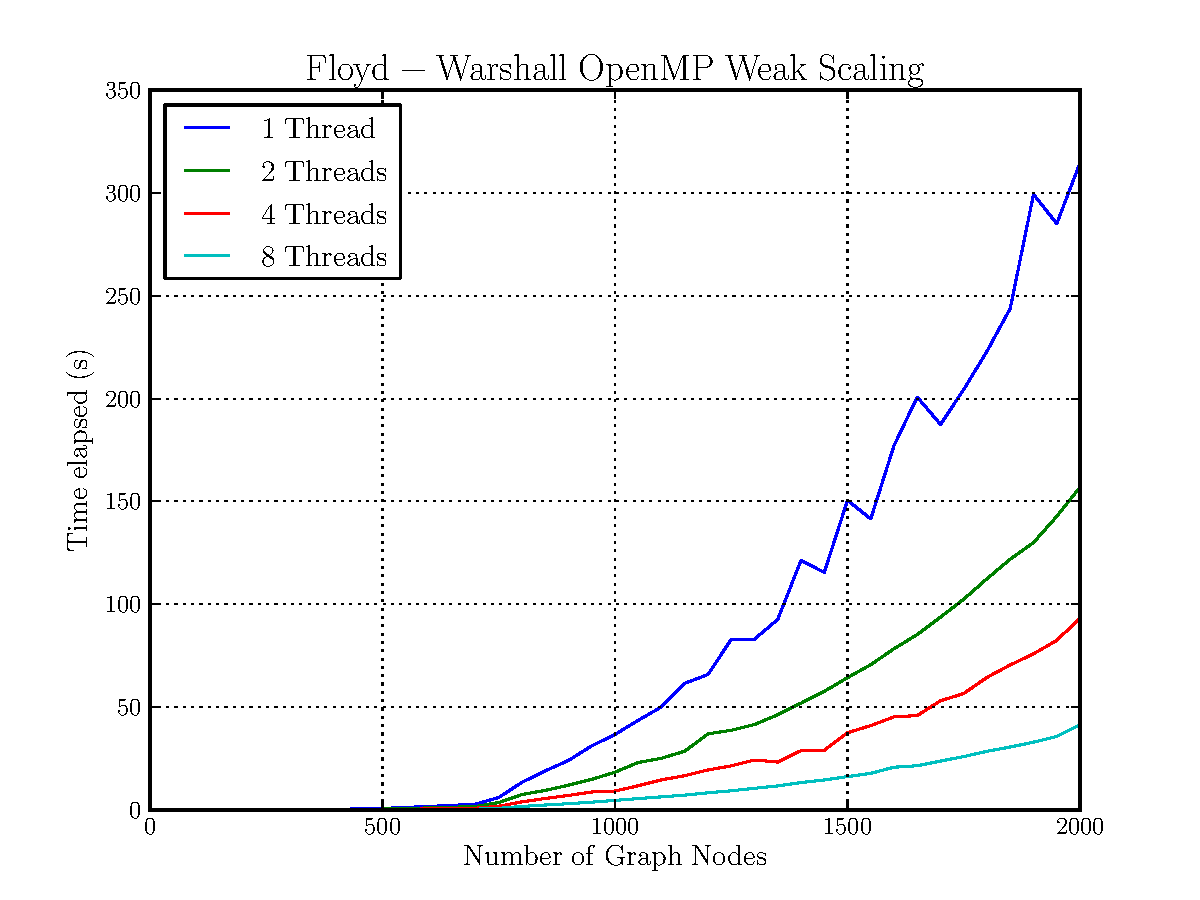
\includegraphics[scale=0.7]{../profiling/omp_linear_weak.pdf}
  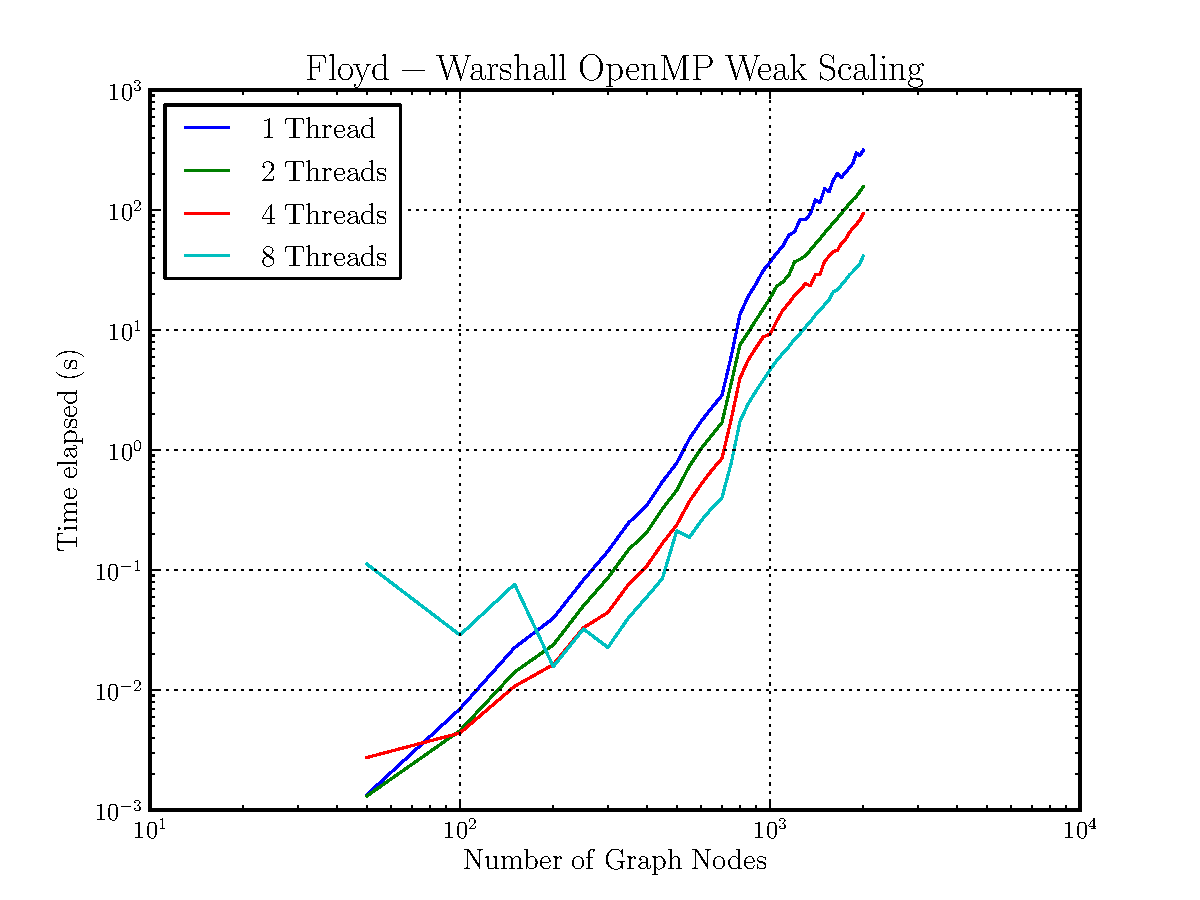
\includegraphics[scale=0.7]{../profiling/omp_log_weak.pdf}
  \caption{Weak scaling results from the reference OpenMP implementation}
\end{figure}

From the logarithmic plot, we observe that as the number of nodes becomes large, the slope of the
plot roughly settles to around three, as we would expect from the $O(n^3 \log n)$ asymptotic
behavior of our algorithm. Curiously, the number of iterations needed per experiment changed
little. Past 200 nodes, each experiment used exactly three iterations. The randomly generated graph
of 50 nodes required five iterations, the most of any graph.

Similarly, we fixed the problem size at 2000 nodes and varied the number of OpenMP threads from one
to eight to collect data for the strong scaling experiment. The ratio between the time taken with one
thread is plotted below.

\begin{figure}
  \centering
  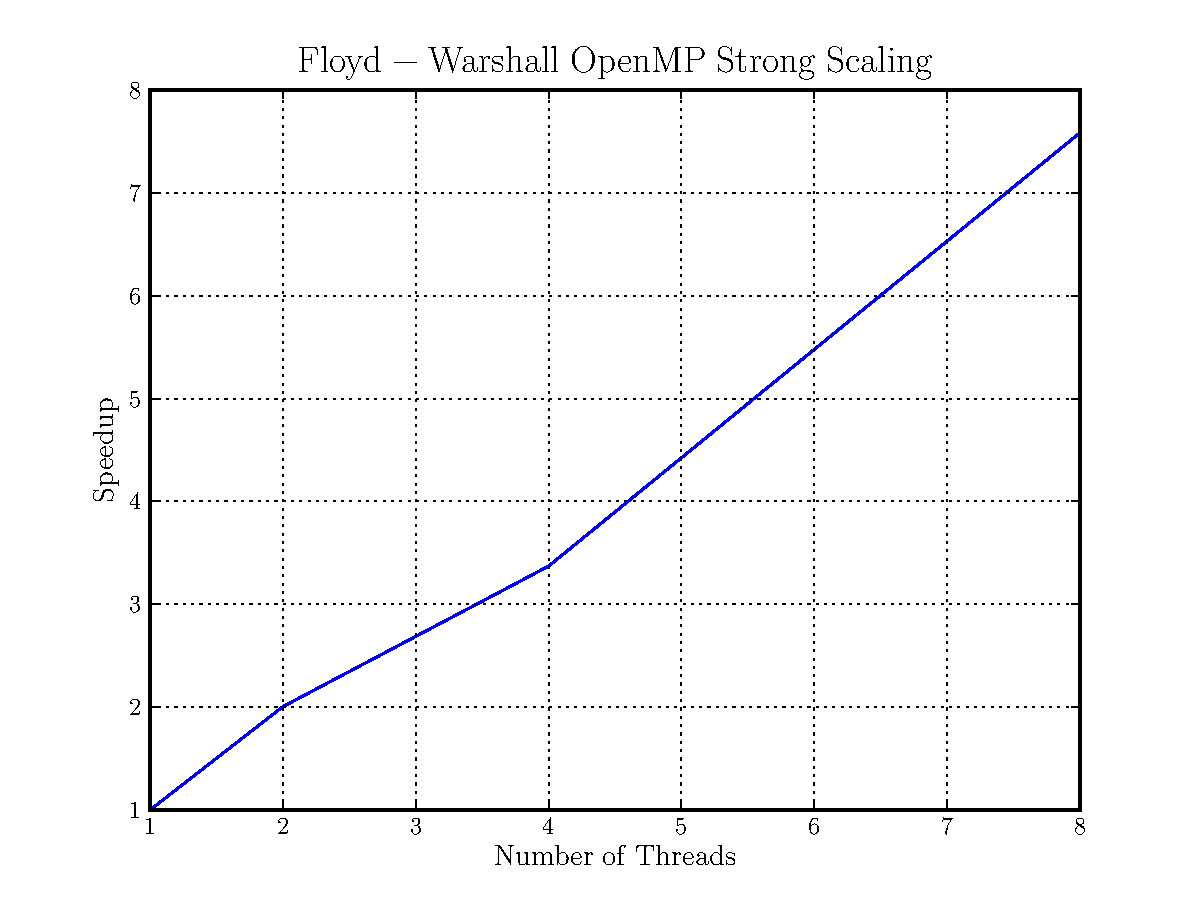
\includegraphics[scale=0.7]{../profiling/omp_strong.pdf}
  \caption{Strong scaling results from the reference OpenMP implementation}
\end{figure}


\end{document}
